\section{Architektur}
Die Architektur beschreibt den allgemeinen Aufbau des Betriebssystems. Eine genaue Beschreibung zu den einzelnen Teilen sind in weiteren Kapiteln in diesem Dokument enthalten.

\subsection{Art des Kernels}
Das Betriebssystem ist ein Monolithischer Kernel. Darunter versteht man einen Kernel, welcher neben Funktionen für Speicherverwaltung, Prozessverwaltung und Kommunikation zwischen Prozessen auch Treiber sowie weitere Komponenten (z.B. Dateisystem) enthält. Durch das Beinhalten dieser Komponenten hat der Monolithische Kernel einen Geschwindigkeitsvorteil gegenüber einem Mikrokernel (Vgl. XXX).
%https://de.wikipedia.org/wiki/Monolithischer_Kernel  
Ein weiterer Grund für einen Monolithischen Kernel ist das entfallen der aufwändigen Kommunikationen zwischen den verschiedenen Komponenten des Betriebssystems.

\subsection{Ansatz für die Abstraktionen im Betriebssystem}
Um eine möglichst gute Abstraktionen im Betriebssystem zu gewährleisten werden Manager für die einzelnen Komponenten verwendet. Eine Übersicht der einzelnen Manager sowie eine bzw. mehrere zugehörige Funktionen, zum besseren Verständnis, ist in Tabelle \ref{table:Manager-function} gegeben. Eine kurze Beschreibung zu den einzelnen Managern ist unter \ref{section:generalArchitecture} gegeben.

\begin{table}[H]
\begin{tabular}{p{4cm} | p{9cm}}
  \textbf{Managername} & \textbf{Beispiel Funktion(en)} \\ 
  \hline
  DeviceManager & InitDevice, OpenDevice, ReadDevice \\
  DriverManager & GetDriver \\
  FileManager & ListDirectoryContent, OpenFile, OpenExecutable \\
  MemManager & GetFreePagesInProcessRegion, GetRegion \\
  ProcessManager & StartProcess, KillProcess, ListProcesses \\
  IpcManager & RegisterNamespace, SendMessage, HasMessage \\
 \end{tabular}
 \caption{Übersicht der Manager mit zugehöriger Funktion}
 \label{table:Manager-function}
\end{table}

\subsection{Allgemeiner Aufbau der Architektur}
\label{section:generalArchitecture}
In Abbildung \ref{fig:general-Architecture} ist der allgemeine Aufbau mit den wesentlichen Teilen der Architektur ersichtlich. 

\begin{figure}[H]
	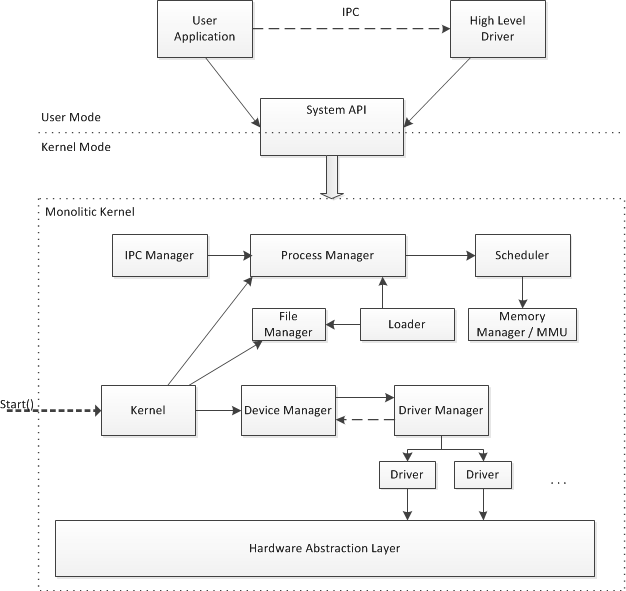
\includegraphics[scale=0.9]{chapters/architecture/figures/architecture}
	\caption{Allgemeiner Aufbau der Architektur}
	\label{fig:general-Architecture}
\end{figure}

Im folgenden wird eine kurze Erläuterung zu den einzelnen Komponenten der Abbildung \ref{fig:general-Architecture} gegeben. Für eine genauere Beschreibung wird auf die einzelnen Kapitel verwiesen. \\

\begin{description}
	\item[Hardware Abstraction Layer (HAL) (Vgl. Kapitel XXX)] \hfill \\
	Der Hardware Abstraction Layer wird, wie der Name bereits beschreibt, zur Abstraktion der Hardware vom eigentlichen Betriebssystem verwendet.
	
	\item[Driver (Vgl. Kapitel XXX)] \hfill \\
	Ein Treiber ist eine abstrakte Schnittstelle zu der Hardware, sodass kein direkter Zugriff auf die HAL benötigt wird.
	
	\item[Driver Manager (Vgl. Kapitel XXX)] \hfill \\
	Der Driver Manager dient zum ansprechen der Treiber, welche vom Betriebssystem zur Verfügung gestellt werden. Sollte ein Treiber benötigt werden, muss dieser nicht erzeugt werden sondern kann über Driver Manager geholt werden. 
	
	\item[Device Manager (Vgl. Kapitel XXX)] \hfill \\
	Der Device Manager dient wie bereits der Driver Manager zur Abstraktion der Treiber. D.h. eine Anwendung verwendet Geräte, welche vom Device Manager zur Verfügung gestellt werden. Ein Beispiel für Devices sind LEDs. Beim Ansprechen einer LED wird ein Treiber benötigt, ohne der Abstraktion auf Geräte müssten bei der Verwendung mehrerer LEDs auch mehrere LED Treiber geschrieben werden oder ein großer Treiber. Der Nachteil eines einzelnen Treibers ist, dass das Ansprechen einzelner LEDs viel Aufwand benötigt.
	
	\item[Kernel (Vgl. Kapitel XXX)] \hfill \\
	Der Kernel ist der Kern des Betriebssystems und enthält das Starten aller Prozesse und Managern. Dazu zählen: Konsole, Device Manager, Driver Manager, Process Manager, File Manager, IPC Manager, etc.
	
	\item[Process Manager (Vgl. Kapitel XXX)] \hfill \\
	Der Process Manager ist zuständig für das Starten und Stoppen (Killen) von Prozessen. Es besteht eine starke Kopplung zum Scheduler.
	
	\item[Scheduler (Vgl. Kapitel XXX)] \hfill \\
	Der Scheduler wechselt die Prozesse in fix definierten Zeitscheiben (10ms). Auch ist das Händeln der verschiedenen Zustände eines Prozesses Aufgabe vom Scheduler. Gültige Zustände sind: Ready, Running, Blocked, Sleeping und Free.
	
	\item[Memory Manager/MMU (Vgl. Kapitel XXX)] \hfill \\
	Über den Memory Manager können freie Pages in der Prozessregion allokiert werden sowie die eine bestehende Region zurückgeliefert werden.

	\item[File Manager (Vgl. Kapitel XXX)] \hfill \\
	Der File Manager dient zum Verarbeiten von dateiabhängigen Operationen. Auflisten der einzelnen Inhalte in einem Verzeichnis, Öffnen einer Datei, Setzen des aktuellen Verzeichnis, etc. sind die Hauptaufgaben dieses Managers.
	
	\item[Loader (Vgl. Kapitel XXX)] \hfill \\
	Der Loader ist dafür zuständig ein existierendes Programm in die Prozessregion zu laden. D.h. der Loader ladet ein auszuführendes Programm in den Speicher, sodass dieses Programm als Prozess ausgeführt werden kann.
	
	\item[IPC Manager (Vgl. Kapitel XXX)] \hfill \\
	Der IPC Manager ist für die Kommunikation zwischen verschiedenen User-Anwendungen zuständig.
	
	\item[System API (Vgl. Kapitel XXX)] \hfill \\
	Die System API stellt eine Schnittstelle für den Anwendungsentwickler/ die Anwendungsentwicklerin zur Verfügung. Dadurch sind die Betriebssystem Funktionen von der Anwendung entkoppelt. Es werden von der Anwendung nur System API Funktionen aufgerufen und keine System Funktionen. Dies führt zu einer höheren Sicherheit des Systems sowie zu einem einfacheren Implementieren von Endanwendungen.
	
	\item[User Application (Vgl. Kapitel XXX)] \hfill \\
	Bei der User Application handelt es sich um das Ansprechen eines Moving Heads mittels DMX Protokoll. Vergleichbare Projekte wären das Ansprechen von Komponenten die zur Kommunikation KNX oder DALI verwenden.
	
	\item[High Level Driver (Vgl. Kapitel XXX)] \hfill \\
	Der High Level Driver ist ein Treiber, welcher dazu dient der eigentlichen BenutzerInnen Anwendung eine verbesserte Schnittstelle zur Verfügung zu stellen. Ansonsten müsste ein Entwickler/ eine Entwicklerin wissen, dass das DMX Protokoll durchgehend sendet, somit wäre in der eigentlichen Anwendung Logik implementiert, welche gar nicht hinein gehört bzw. davon abstrahiert gehört.
\end{description}

\pagebreak 